\documentclass[11pt]{article}
\usepackage{geometry}                
\geometry{letterpaper}                   

\usepackage{graphicx}
\usepackage{amssymb}
\usepackage{epstopdf}
\usepackage{natbib}
\usepackage{amssymb, amsmath}
\DeclareGraphicsRule{.tif}{png}{.png}{`convert #1 `dirname #1`/`basename #1 .tif`.png}

%\title{Title}
%\author{Name 1, Name 2}
%\date{date} 

\begin{document}



\thispagestyle{empty}

\begin{center}
\includegraphics[width=5cm]{ETHlogo.eps}

\bigskip


\bigskip


\bigskip


\LARGE{ 	Lecture with Computer Exercises:\\ }
\LARGE{ Modelling and Simulating Social Systems with MATLAB\\}

\bigskip

\bigskip

\small{Project Report}\\

\bigskip

\bigskip

\bigskip

\bigskip


\begin{tabular}{|c|}
\hline
\\
\textbf{\LARGE{Zurich traffic simulation Sihlstrasse/Uraniastrasse}}\\
\\
\hline
\end{tabular}
\bigskip

\bigskip

\bigskip

\LARGE{Filip Meier \& Sebastian Honegger}



\bigskip

\bigskip

\bigskip

\bigskip

\bigskip

\bigskip

\bigskip

\bigskip

Zurich\\
December 2015\\

\end{center}



\newpage

%%%%%%%%%%%%%%%%%%%%%%%%%%%%%%%%%%%%%%%%%%%%%%%%%

\newpage
\section*{Agreement for free-download}
\bigskip


\bigskip


\large We hereby agree to make our source code for this project freely available for download from the web pages of the SOMS chair. Furthermore, we assure that all source code is written by ourselves and is not violating any copyright restrictions.

\begin{center}

\bigskip


\bigskip


\begin{tabular}{@{}p{3.3cm}@{}p{6cm}@{}@{}p{6cm}@{}}
\begin{minipage}{3cm}

\end{minipage}
&
\begin{minipage}{6cm}
\vspace{2mm} \large Name 1

 \vspace{\baselineskip}

\end{minipage}
&
\begin{minipage}{6cm}

\large Name 2

\end{minipage}
\end{tabular}


\end{center}
\newpage

%%%%%%%%%%%%%%%%%%%%%%%%%%%%%%%%%%%%%%%



% IMPORTANT
% you MUST include the ETH declaration of originality here; it is available for download on the course website or at http://www.ethz.ch/faculty/exams/plagiarism/index_EN; it can be printed as pdf and should be filled out in handwriting


%%%%%%%%%% Table of content %%%%%%%%%%%%%%%%%

\tableofcontents

\newpage

%%%%%%%%%%%%%%%%%%%%%%%%%%%%%%%%%%%%%%%



\section{Abstract}

\section{Individual contributions}

\section{Introduction and Motivations}


The city of Zurich planing to change one specific part of the sihlstrasse in a pedestrian area. The idea is to make this area more comfortable for the visitors of the city center and it should be also an upgrade for the restaurants and shops around this area.
\begin{figure}[h]
\begin{minipage}[t]{.45\textwidth}
	\centering
	\vspace{30pt}
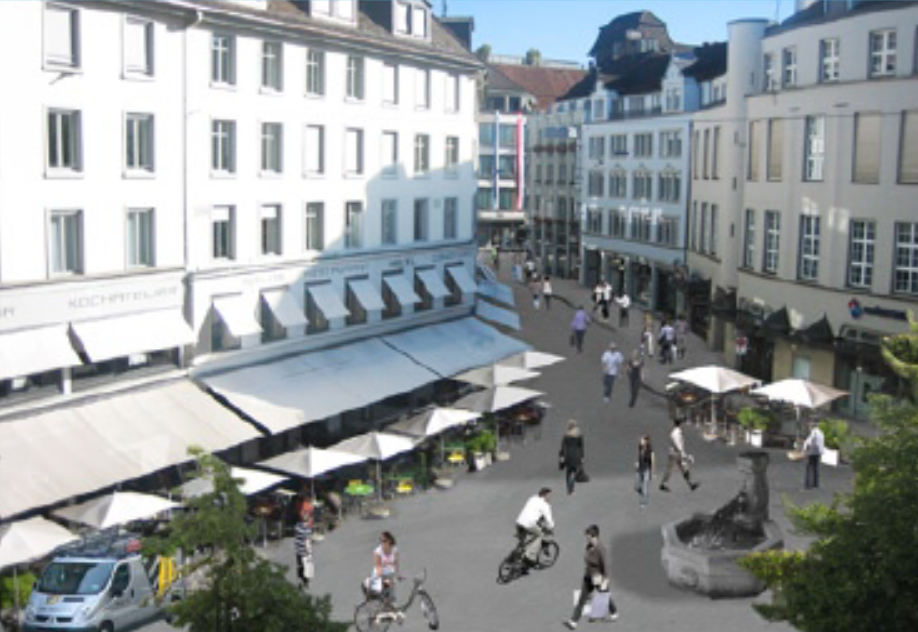
\includegraphics[width=\textwidth]{pedestrianarea.png}
\end{minipage}\hfill
\begin{minipage}[t]{.45\textwidth}
	\centering
	\vspace{0pt}
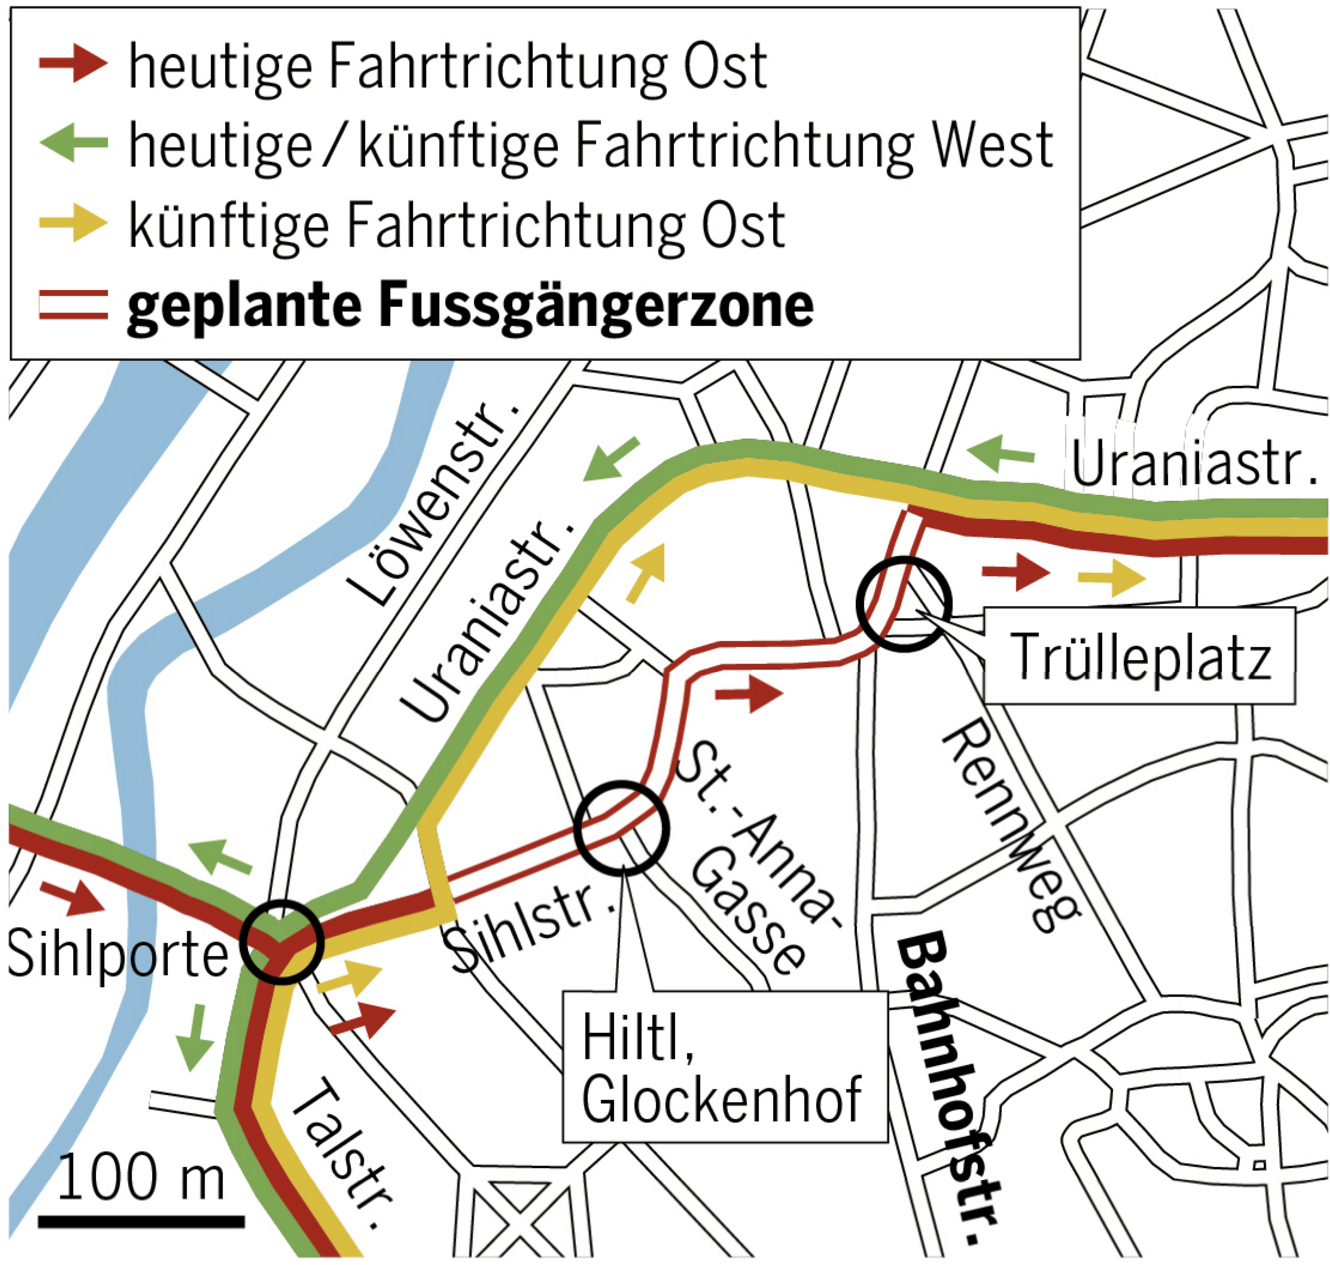
\includegraphics[width=\textwidth]{Plan_Sihlstrasse.png}
\end{minipage}\hfill
\caption{right: situation plan which shows the change of the tracks. left: illustraion of the pedestrian area at sihlstrasse.}
\end{figure}
\\
The changet will have a big impact for the traffic because there will be one track less than before. Sihlstrasse (from west to east) and Uraniastrasse (from east to west) is one of the most travelled  road in the city center. It is the only alternative road to the highway (Westumfarung). If they decide to built a pedestrian area in the sihlstrasse they will lose one track from west to east.
We know want to analyse the impact to the traffic jam and the impact on the neighbourhood streets.

\section{Fundamental Questions}

With our simulation, we want to answered the following questions:
\begin{itemize}
\item[1.] Are the streets still large enough to manage the traffic jam peaks on working days?
\item[2.] What is the impact on the neigbourhood streets?
\item[3.] Which area or signal light is the bottleneck?
\end{itemize}
\section{Description of the Model}

\section{Implementation}

\section{Simulation Results and Discussion}

\section{Summary and Outlook}

\section{References}






\end{document}  



 
